% Appendix G: the released remap. Input by sections/appendix.tex.
\section{The released remap}\label{app:remap}\label{sec:intervention}

This appendix describes, in our words, the intervention released with \citet{anonymous2026fitted} and everything we measured on it: the reproduction, the crossover across formats that motivates \cref{sec:claim3}, the refit without later mentions (preregistration F), the reader heads at 24B under the remap (preregistration I) and the same frames under the emitted-form score (final round). All of it is discovery sample except the last part. We describe what the released analysis does, not what its authors concluded from it.

\subsection{What the released analysis does}\label{app:remap-what}

The released analysis of \citet{anonymous2026fitted} patches Mistral-Small-24B and Qwen2.5-72B at the output of (1-based) decoder block 4 over every token of the event span (from ``\{$A$\} watches as'' to the end of the story). For a rank-16 basis $U$ with orthonormal rows, each span position becomes
\begin{equation}\label{eq:patch}
h \leftarrow h_{\mathrm{B}} + U^{\top} U\,(h_{\mathrm{S}} - h_{\mathrm{B}}).
\end{equation}
In the learned remap M, $U$ is a distributed alignment search basis \citep{geiger2024finding} fit with a six-choice cross-entropy objective so that the patched model ranks $\mathrm{T} = \pi(\mathrm{S})$ first, where $\pi$ is a fixed pair-swap of the six locations. In the control P, $U$ is an unfitted PCA basis of source-minus-base differences, which transfers S. We reuse the released bases (three seeds each; the Qwen2.5-72B PCA bases are reconstructions, labelled so by \citet{anonymous2026fitted}). Following the released design, a \emph{key-only exchange} replaces the writing token's key in every block from (1-based) block 6 on by the key of the other patched run, while queries, values and residual states evolve freely; we add the symmetric \emph{value-only exchange}. Unlike our clamp, these exchanges are not exact, because the patch also changes the other span tokens. With $m_{\mathrm{TS}} = \log p(\mathrm{T}) - \log p(\mathrm{S})$, writing $\mathrm{P}{+}K_{\mathrm{M}}$ for P with M's keys and $m(\cdot)$ for $m_{\mathrm{TS}}$ in a run,
\begin{align}
\varphi &= \frac{m(\mathrm{M}) - m(\mathrm{P})}{m(\mathrm{T}) - m(\mathrm{S})}, \label{eq:phi}\\
\psi_K &= \frac{m(\mathrm{P}{+}K_{\mathrm{M}}) - m(\mathrm{P})}{m(\mathrm{M}) - m(\mathrm{P})}, \label{eq:psik}\\
\psi_V &= \frac{m(\mathrm{P}{+}V_{\mathrm{M}}) - m(\mathrm{P})}{m(\mathrm{M}) - m(\mathrm{P})}. \label{eq:psiv}
\end{align}
$\varphi$ is the shift of M beyond P towards T, as a fraction of the natural S$\to$T shift; $\psi_K$ and $\psi_V$ are the fractions of the learned-minus-PCA difference that M's keys or values add to P. All are ratios of means over the 96 of their 120 native story cores in which B, S and T are distinct, after averaging the three fits within each core.

The exchanges are not exact, because the patch also changes the other span tokens; the removal fractions $\chi_K$ and $\chi_V$ and the implementation are in \cref{app:impl-clamps}. The remap was fit without the ``Answer:'' prefill of our formats, which the released analysis adds only at evaluation.

\subsection{Reproduction and the crossover across formats}\label{app:remap-crossover}

\paragraph{Reproduction.} Under \fmtOpt{}, the format of the released analysis, our runs of the released bases reproduce the released answers: the argmax of M and of P agrees with the released outputs on 0.994--1.000 of (core, fit) items (a preregistered gate, \cref{tab:prereg-c}). As in the released analysis, M's keys alone reproduce a substantial part of the M$-$P difference in both models ($\psi_K$ = \psiOptMistral{} and \psiOptQwen{} under \fmtOpt{}), and, in a comparison the release does not make, more of it than M's values do. We did not re-test the release's colour-lookup questions, and we score log-odds where the release scores argmax agreement. The addition fractions sum to less than one and the removal fractions mostly to more than one (\cref{tab:frames}), so the channels do not combine additively, and part of the edit may travel through the other patched span tokens. % verbatim: 0.994--1.000, outcome of C

\begin{figure}[!ht]
  \centering
  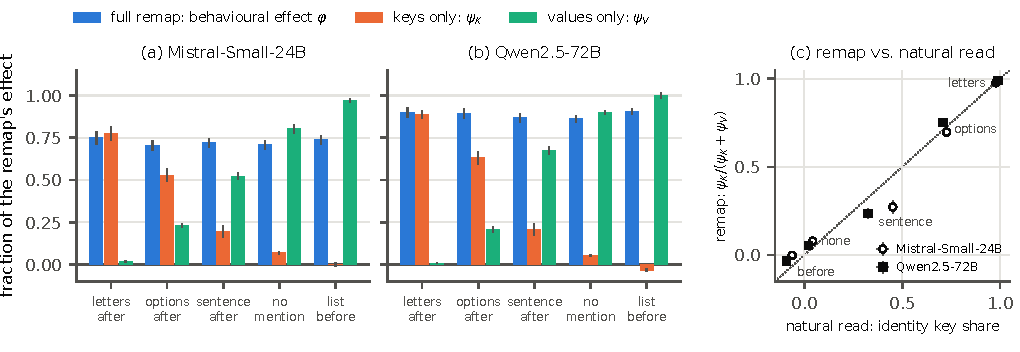
\includegraphics[width=\textwidth]{figures/fig_frames.pdf}
  \caption{\textbf{The same learned intervention has nearly the same behavioural effect in every format, but whether the writing token's keys or values carry it depends on the later mentions} (discovery sample). The released remap M of \citet{anonymous2026fitted} against the PCA patch P at Mistral-Small-24B (a) and Qwen2.5-72B (b): $\varphi$, $\psi_K$ and $\psi_V$ (\cref{eq:phi,eq:psik,eq:psiv}), exchanged from block~6 on; $n = 96$ cores $\times$ 3 fits, 95\% bootstrap intervals. (c)~The remap's key share $\psi_K/(\psi_K+\psi_V)$ against the unpatched model's $s_{\mathrm{ID}}$ in the same format: post hoc for the released remaps, preregistered (F4) for the refits (triangles; \cref{app:refit}). Diamonds: the binding swap of \citet{prakash2025lookbacks} at Qwen2.5-14B, $\kappa$ at block $\ell^*$ against $s_{\mathrm{ID}}$ from block $\ell^*{+}1$ (H7, failed); crosses: the identity edit at block~0 against $s_{\mathrm{ID}}$ from block~1 (H11, met). Values in \cref{tab:frames,tab:refit,tab:prakash}.}
  \label{fig:frames}
\end{figure}

\paragraph{Behaviour barely changes across formats; the carrying channel flips.} We then changed only the format and added a value-only exchange. Two comparisons are confirmatory and met in both models: without a later mention M's keys carry less than half of what they carry under \fmtOpt{} (C3), and M's values carry most of the effect (E4). $\varphi$ lies between \phiOptMistral{} and \phiLetterMistral{} at Mistral-Small-24B and between \phiNoneQwen{} and \phiBeforeQwen{} at Qwen2.5-72B, and the PCA control transfers the source location in every format. Yet at Qwen2.5-72B, M's keys reproduce \psiLetterQwen{} of the M$-$P difference under \fmtLetter{} but \psiNoneQwen{} under \fmtNone{}, while M's values do the reverse (\cref{fig:frames}b). Mistral-Small-24B and the removal fractions show the same crossover. Across the ten format--model cells, the remap's key share tracks the identity key share $s_{\mathrm{ID}}$ of the unpatched model in the same format (\cref{fig:frames}c; $r = \crossR{}$): post hoc for the released remaps, preregistered for the refits (\cref{app:refit}), and failed out of sample for a binding edit (\cref{app:binding}).

\paragraph{Interpretation (post hoc, discovery sample).} In \fmtLetter{}, \fmtOpt{}, \fmtPost{} and \fmtNone{} the prompt is identical up to the end of the story, so under the causal mask M writes the same key and the same value at the writing token in all four; only their readers differ, and which channel appears to carry the edit follows them. Its value half (E4) and the refit test (F) were then preregistered and confirmed. Whether this reading extends to edits obtained independently of the released remap is the channel-ratio law of the final round, which failed (\cref{sec:claim3,app:claim3}).

\paragraph{Intervention frames.} \Cref{tab:frames} gives every frame quantity with its interval. At Qwen2.5-72B, M's keys reproduce \psiLetterQwen{} of the M$-$P difference under \fmtLetter{} and \psiOptQwen{} under \fmtOpt{}, but only \psiPostQwen{} under \fmtPost{}, \psiNoneQwen{} under \fmtNone{} and $\psiBeforeQwen$ under \fmtBefore{}, while M's values do the reverse ($\psi_V$ = \psiVLetterQwen{}, \psiVOptQwen{}, \psiVPostQwen{}, \psiVNoneQwen{}, \psiVBeforeQwen{}; exploratory except C3 and E4). The removal fractions follow the addition fractions: $\chi_K$ is large where $\psi_K$ is, and $\chi_V$ where $\psi_V$ is. Among the six candidates, M's top answer is the target T in \mTLetterMistral{}--\mTPostMistral{} of (core, fit) items at Mistral-Small-24B and \mTNoneQwen{}--\mTBeforeQwen{} at Qwen2.5-72B, depending on the format.

\begin{table}[!ht]
\centering
\caption{\textbf{The intervention of \citet{anonymous2026fitted} across formats.} $\varphi$: behavioural shift of the learned remap M relative to the PCA patch P, as a fraction of the natural source-to-target shift (\cref{eq:phi}). $\psi_K$, $\psi_V$: fraction of the M$-$P difference that P reproduces when given M's keys or values at the writing token (\cref{eq:psik,eq:psiv}). $\chi_K$, $\chi_V$: fraction of that difference that M loses when given P's keys or values (\cref{app:impl}). Exchanges from block~6 on. $n = 96$ story cores with B, S and T distinct, three fits averaged within each core; 95\% bootstrap CIs over cores. Preregistrations C (C1--C3) and E (E4) for the cells they name; the rest exploratory.}
\label{tab:frames}
\resizebox{\textwidth}{!}{\begin{tabular}{llccccc}
\toprule
Model & Format & $\varphi$ & $\psi_K$ & $\chi_K$ & $\psi_V$ & $\chi_V$ \\
\midrule
Mistral-Small-24B & \fmtLetter{} & 0.75 [0.71, 0.79] & 0.78 [0.73, 0.82] & 0.99 [0.98, 0.99] & 0.02 [0.01, 0.02] & 0.16 [0.13, 0.19] \\
 & \fmtOpt{} & 0.70 [0.68, 0.73] & 0.53 [0.49, 0.57] & 0.76 [0.75, 0.78] & 0.23 [0.22, 0.24] & 0.44 [0.41, 0.48] \\
 & \fmtPost{} & 0.72 [0.69, 0.75] & 0.20 [0.16, 0.23] & 0.45 [0.43, 0.47] & 0.52 [0.50, 0.54] & 0.77 [0.73, 0.81] \\
 & \fmtNone{} & 0.71 [0.68, 0.73] & 0.07 [0.06, 0.08] & 0.18 [0.16, 0.20] & 0.80 [0.78, 0.83] & 0.93 [0.92, 0.94] \\
 & \fmtBefore{} & 0.74 [0.71, 0.76] & -0.00 [-0.01, 0.01] & 0.01 [-0.00, 0.02] & 0.97 [0.96, 0.98] & 0.96 [0.95, 0.98] \\
\midrule
Qwen2.5-72B & \fmtLetter{} & 0.90 [0.87, 0.93] & 0.89 [0.86, 0.91] & 0.99 [0.99, 1.00] & 0.01 [0.00, 0.01] & 0.17 [0.13, 0.20] \\
 & \fmtOpt{} & 0.89 [0.86, 0.92] & 0.63 [0.59, 0.67] & 0.79 [0.78, 0.81] & 0.21 [0.19, 0.23] & 0.44 [0.39, 0.48] \\
 & \fmtPost{} & 0.87 [0.84, 0.89] & 0.21 [0.17, 0.25] & 0.34 [0.31, 0.36] & 0.67 [0.65, 0.70] & 0.80 [0.76, 0.84] \\
 & \fmtNone{} & 0.86 [0.84, 0.88] & 0.05 [0.05, 0.06] & 0.11 [0.09, 0.12] & 0.90 [0.88, 0.91] & 0.95 [0.94, 0.96] \\
 & \fmtBefore{} & 0.91 [0.88, 0.92] & -0.03 [-0.04, -0.02] & -0.02 [-0.04, -0.01] & 1.00 [0.98, 1.01] & 1.01 [0.99, 1.02] \\
\bottomrule
\end{tabular}
}
\end{table}

\subsection{A remap fit without later mentions (preregistration F)}\label{app:refit}\label{sec:refit}

The remap edits block 4, upstream of every exchanged key and value. Preregistration F asked whether the format it was fit in, rather than its readers, decides its channel: at Mistral-Small-24B it refit the remap with the released code under \fmtNone{} (fit\_none) and, as a same-code control, under \fmtOpt{} (fit\_opt). All gates and all four predictions were met (\cref{tab:prereg-f,tab:refit}): fit\_none is carried by keys under \fmtLetter{} ($\psi_K = \psiLetterRefNone{}$) and by values under \fmtNone{} ($\psi_V = \psiVNoneRefNone{}$), transfers to lettered options ($\varphi = \phiLetterRefNone{}$), shows the control's crossover (F3), and its key share tracks the natural read ($r = \refRNone{}$; \cref{fig:frames}c). The reading format decides which channel dominates.

\paragraph{Recipe.} We ran the released training code of \citet{anonymous2026fitted} (\texttt{gpu/train.py} and \texttt{gpu/behavior\_engine.py}, unmodified) through \texttt{experiments/refit\_remap.py}. Its recipe: a rank-16 basis at the output of (1-based) block 4 over every event-span token; the pair-swap objective with a six-way conditional cross-entropy at the start of the reply (no prefill); AdamW, learning rate $10^{-3}$, batch 1, one shuffled epoch of their 1000 training pairs (2000 stories); seeds 101--103, which change only the order of the training pairs: every fit starts from the same PCA basis of source-minus-base differences (the randomised sketch differs by seed but returns the same subspace, mean squared principal cosine \refPcaSame{} across seeds), and that basis is the control P of every fit. The code also fits an identity-objective basis next to each remap (exploratory): its shift of the answer towards T, relative to P and as a fraction of the natural S$\to$T shift, is at most \refFstarMaxNone{} for fit\_none (under \fmtLetter{}) and \refFstarMaxOpt{} for fit\_opt. The training stories are disjoint from the 120 evaluation cores, but most evaluation event sentences also occur in some training story, as for the released remap.

\paragraph{What the wrapper replaces.} At import time, and recorded with hashes in each run's \texttt{FRAME.json}: the prompt function, for fit\_none only, by our \fmtNone{} prompt, which agrees token for token with the original prompt up to the end of the story in all 1000 training pairs; the release-integrity check, by one that tolerates only the release's mismatched \texttt{README.md}; and the model loader, by one with the same load arguments (BF16, sdpa, eval mode, no gradients, no cache, pad = eos, \texttt{fix\_mistral\_regex}) at the pinned revision, waiving the release's exact Python, package, device and memory pins and its model-asset receipt (the weights are identified instead by the pinned commit, which the loader checks). Under the causal mask the activations up to the end of the story are the same in both runs, so both start from the same P; the PCA bases came out bitwise identical across runs.

\paragraph{Results.} \Cref{tab:refit} gives every frame quantity for the two refits and for the released bases re-run in the same job; \cref{tab:prereg-f} gives the gates and predictions. The rest of this paragraph is exploratory. The control matches the released remap to within \refMaxDiffOpt{} in every quantity and format. Every fitted remap keeps \refCosFloorMin{}--\refCosFloorMax{} of its subspace (mean squared principal cosine) in the shared PCA start, against \refCosChance{} for random subspaces, so overlaps between fits lie above that floor: fit\_opt overlaps the released remap at \refCosOptMin{}--\refCosOptMax{}, while fit\_none overlaps the released remap at \refCosNoneMin{}--\refCosNoneMax{} and fit\_opt at \refCosNoneOptMin{}--\refCosNoneOptMax{}, less than two seeds of one fit overlap each other (\refCosSeedMin{}--\refCosSeedMax{}). Without the ``Answer:'' prefill, which matches the interface the remaps were fit at, the difference in differences is $\refDNoPre{}$ [$\refDNoPreLo{}$, $\refDNoPreHi{}$]. The training loss of the remap fits fell from \refLossFirstMin{}--\refLossFirstMax{} nats over the first 100 updates to \refLossLastMin{}--\refLossLastMax{} over the last 100; it starts above chance ($\ln 6 \approx 1.79$) because the PCA start transfers the source, which the pair-swap objective scores as wrong.

\paragraph{Where the fitting format still matters (post hoc).} The fitting format shifts the balance where both channels read, in the direction the stated alternative predicts. fit\_none's $\psi_K$ is lower than the control's by \refDiffOpt{} [\refDiffLoOpt{}, \refDiffHiOpt{}] under \fmtOpt{} and by \refDiffPost{} [\refDiffLoPost{}, \refDiffHiPost{}] under \fmtPost{}. It transfers better under \fmtNone{} ($\varphi = \phiNoneRefNone{}$ against \phiNoneRefOpt{}) and worse under \fmtLetter{} (\phiLetterRefNone{} against \phiLetterRefOpt{}), where its values carry almost nothing ($\psi_V = \psiVLetterRefNone{}$). These comparisons were made after seeing the data; the preregistered all-or-none alternative (\cref{tab:prereg-f}) was not observed.

\begin{table}[!ht]
\centering
\footnotesize
\caption{\textbf{Refit remaps in the frames of \citet{anonymous2026fitted}} (Mistral-Small-24B, ``Answer:'' prefill). fit\_none: refit under \fmtNone{}; fit\_opt: refit under \fmtOpt{} with the same code; released: the released bases, re-run in the same job. All fits share one PCA control P. $n = 96$ cores, three fits averaged within core; 95\% core bootstrap.}
\label{tab:refit}
{\setlength{\tabcolsep}{4pt}\begin{tabular}{llccccc}
\toprule
Remap & Format & $\varphi$ & $\psi_K$ & $\chi_K$ & $\psi_V$ & $\chi_V$ \\
\midrule
fit\_none & \fmtLetter{} & 0.67 [0.64, 0.70] & 0.77 [0.73, 0.80] & 0.98 [0.97, 0.98] & 0.02 [0.02, 0.03] & 0.15 [0.13, 0.19] \\
 & \fmtOpt{} & 0.72 [0.70, 0.74] & 0.43 [0.39, 0.47] & 0.74 [0.73, 0.76] & 0.25 [0.23, 0.26] & 0.54 [0.50, 0.58] \\
 & \fmtPost{} & 0.81 [0.79, 0.83] & 0.12 [0.10, 0.15] & 0.47 [0.44, 0.49] & 0.50 [0.47, 0.52] & 0.85 [0.81, 0.88] \\
 & \fmtNone{} & 0.81 [0.79, 0.84] & 0.07 [0.06, 0.08] & 0.18 [0.16, 0.20] & 0.80 [0.77, 0.82] & 0.93 [0.91, 0.94] \\
 & \fmtBefore{} & 0.76 [0.74, 0.78] & 0.01 [0.00, 0.02] & 0.00 [$-$0.01, 0.01] & 0.97 [0.96, 0.99] & 0.95 [0.94, 0.96] \\
\midrule
fit\_opt & \fmtLetter{} & 0.77 [0.74, 0.80] & 0.78 [0.73, 0.82] & 0.98 [0.98, 0.99] & 0.02 [0.01, 0.02] & 0.16 [0.13, 0.19] \\
 & \fmtOpt{} & 0.72 [0.69, 0.74] & 0.52 [0.48, 0.56] & 0.76 [0.74, 0.77] & 0.23 [0.22, 0.24] & 0.44 [0.40, 0.48] \\
 & \fmtPost{} & 0.73 [0.71, 0.75] & 0.20 [0.16, 0.23] & 0.45 [0.43, 0.47] & 0.52 [0.50, 0.54] & 0.77 [0.73, 0.81] \\
 & \fmtNone{} & 0.72 [0.69, 0.74] & 0.07 [0.06, 0.08] & 0.17 [0.15, 0.19] & 0.81 [0.78, 0.83] & 0.93 [0.92, 0.94] \\
 & \fmtBefore{} & 0.77 [0.74, 0.79] & 0.00 [$-$0.01, 0.01] & 0.00 [$-$0.01, 0.02] & 0.98 [0.96, 0.99] & 0.96 [0.95, 0.98] \\
\midrule
released & \fmtLetter{} & 0.75 [0.71, 0.79] & 0.78 [0.74, 0.82] & 0.99 [0.98, 0.99] & 0.02 [0.01, 0.02] & 0.16 [0.13, 0.19] \\
 & \fmtOpt{} & 0.70 [0.68, 0.73] & 0.53 [0.49, 0.57] & 0.76 [0.75, 0.78] & 0.23 [0.22, 0.24] & 0.44 [0.41, 0.48] \\
 & \fmtPost{} & 0.72 [0.69, 0.75] & 0.20 [0.16, 0.23] & 0.45 [0.43, 0.47] & 0.52 [0.50, 0.54] & 0.77 [0.73, 0.81] \\
 & \fmtNone{} & 0.71 [0.68, 0.73] & 0.07 [0.06, 0.08] & 0.18 [0.16, 0.20] & 0.80 [0.78, 0.83] & 0.93 [0.92, 0.94] \\
 & \fmtBefore{} & 0.74 [0.71, 0.76] & 0.00 [$-$0.01, 0.01] & 0.01 [0.00, 0.02] & 0.97 [0.96, 0.98] & 0.96 [0.95, 0.98] \\
\bottomrule
\end{tabular}
}
\end{table}

\subsection{The reader heads at 24B under the remap (preregistration I)}\label{app:stage7}\label{sec:link}

Preregistration I (GPU stage 7; \cref{tab:prereg-i}) was written because the two halves of the paper were linked only by inference: the reader heads were shown at two 7B models (\cref{app:heads}), the format dependence of the remap at 24B and 72B (\cref{app:remap-crossover}). It tests the link at Mistral-Small-24B on the 96 cores and released bases of the frames (\cref{tab:frames}), with M and its PCA control P patched at block 4 and the key or value of the writing token exchanged from block 6, as there.

\paragraph{The readers at 24B (Gate I-G2).} Heads are ranked by $a_3$ (\cref{app:heads}) on 60 ranking stories that share no story with the 96 cores, separately for each format, with the natural key clamped at the writing token from block~6, where the exchange starts; heads in blocks 1--5 cannot see the exchanged key and are not eligible (1120 of the 1280 heads remain). $H^*$ is the top \Ikstar{}, 5\% of all heads. On the 96 cores the option rows carry \IgtwoRatioOpt{}, \IgtwoRatioLetter{} and \IgtwoRatioPost{} of the natural key effect under \fmtOpt{}, \fmtLetter{} and \fmtPost{}. $H^*$ alone recovers $R(64)$ = \IgtwoROpt{}, \IgtwoRLetter{} and \IgtwoRPost{} of the option rows' read, and blinding $H^*$ removes $\mathrm{KO}(64)$ = \IgtwoKOOpt{}, \IgtwoKOLetter{} and \IgtwoKOPost{}; random sets of 64 recover at most \IgtwoRrandPost{} and remove at most \IgtwoKOrandPost{} (means of three). $R(64)$ is lower than at 7B only on a story type the ranking stories lack, the \InDist{} of the 96 cores whose distractor location equals B or S: on the other cores $R(64)$ = \IrSixtyfourRestOpt{}, \IrSixtyfourRestLetter{} and \IrSixtyfourRestPost{}, on those \IrSixtyfourDistOpt{}, \IrSixtyfourDistLetter{} and \IrSixtyfourDistPost{} (exploratory, recomputed, exploratory). Also exploratory: the sets of \fmtOpt{} and \fmtLetter{} share \IxOverlapOptLetter{} of 64 heads, those of \fmtOpt{} and \fmtPost{} \IxOverlapOptPost{}; ranking heads on the remap itself (P against P with M's key, in-sample on the 96 cores) gives sets that share \IremOverlapOpt{}, \IremOverlapLetter{} and \IremOverlapPost{} heads with $H^*$.

\paragraph{The remap's key read (I1--I3).} In the exchange-blinding operation, chosen heads at the option rows see P's own key at the writing token instead of M's, pinned from block 6, while every other head and row sees M's key. Blinding every head at the option rows removes $g_K$ = \IoneGOpt{} and \IoneGLetter{} of M's key-only effect (\IoneGPost{} under \fmtPost{}, reported). Blinding only $H^*$ removes \ItwoKOOpt{} and \ItwoKOLetter{} of that read (\ItwoKOPost{}), and random or active-at-$G$ sets at most \IthreeMax{}. Little of M's key effect is read outside the option rows: the key route of about one nat seen without a later mention does not persist when the candidates are mentioned, which is why some ratios against \fmtNone{} exceed 1 (\cref{app:prereg}).

\paragraph{Ablation and knockout (I4--I7).} \Cref{tab:link} gives every condition. The ablation A replaces each head's output at the option rows by its mean over the ranking stories, in every row of the frames batch, as in H3; A$^+$ adds the 32 heads of block 5; the knockout N stops the heads from attending from the option rows to the writing token. Under \fmtOpt{}, A($H^*$) removes nearly all of M's key-only effect, moves its key share near its \fmtNone{} level (I4) and raises its value-only effect by \IfiveDV{} nats, \IfiveRatio{} of the lost key effect (I5). The non-additive part of M's effect ($D - K - V$, which also holds reads of the other patched span tokens and, in block 5, of the writing token) falls from \InonAddU{} to \InonAddA{} nats (exploratory, recomputed), and $t$ = \IsixT{}. Post hoc, most of the fall in $D = m(\mathrm{M}) - m(\mathrm{P})$ is in P's rows: ablating the readers compresses every margin, so $m(\mathrm{P})$ rises from $\ImPU$ to $\ImPA$ nats while $m(\mathrm{M})$ falls only from \ImMU{} to \ImMA{}, and the unedited model's margin for its own answer over S falls from \IbMarginU{} to \IbMarginA{} nats while that answer stays the top one in every core. Under \fmtLetter{} (reported two-sided) the remap and the natural task both lose: $t$ = \IsixTLetter{}, M's target is the top answer in \IsixMTALetter{} of cases (\IsixMTLetter{} unblocked) and the natural answer in \IsixBBALetter{} of cores, consistent with the entry's caution that a lettered answer may need the readers. Under \fmtPost{} every threshold is met ($t$ = \IsixTPost{}; reported). The knockout N($H^*$) keeps more of M's effect than the ablation under \fmtOpt{} ($t$ = \InTOpt{}), and less under \fmtLetter{} ($t$ = \InTLetter{}), where answers move to the initial location in about a fifth of cases, as with the all-heads knockout at Qwen2.5-7B (G7).

\begin{table}[!ht]
\centering
\footnotesize
\caption{\textbf{The remap under each blocking at Mistral-Small-24B} (preregistration I; values as printed by the scorer). $t = D^O/D^\emptyset$; superscripts $O$ and $\emptyset$: with and without the blocking; $\kappa = K/(K+V)$ with the $\kappa$ rule (--: $\kappa$ undefined in 99\% of resamples; $\Delta_V$ not applicable or M$\to$T not printed); $\tilde\psi_K = K^O/D^\emptyset$ and $\tilde\psi_V = V^O/D^\emptyset$; $\Delta_V = V^O - V^\emptyset$, paired by core; $D$, $K$, $V$: M's effect, its key-only and its value-only part, in nats; M$\to$T: share of (core, fit) items whose top answer is M's target. A: mean-ablation of the heads' outputs at the option rows; A$^+$: with block 5; N: no attention from the option rows to the writing token. $^\dagger$Exploratory: N(all at $G$), every head at the option rows $G$; A(block 5), the 32 heads of block 5 alone; N(rand0), the first random set of 64; A($H^*_{\text{\fmtOpt{}}}$), the \fmtOpt{} set ablated under \fmtLetter{}. 95\% core-bootstrap CIs.}
\label{tab:link}
{\scriptsize\setlength{\tabcolsep}{3pt}\begin{tabular}{@{}llccccccc@{}}
\toprule
Format & Condition & $t$ & $\kappa$ & $\tilde\psi_K$ & $\tilde\psi_V$ & $\Delta_V$ (nats) & $D$ / $K$ / $V$ (nats) & M$\to$T \\
\midrule
\fmtOpt{} & unblocked & 1 & 0.698 & 0.528 & 0.229 & -- & 13.67 / 7.22 / 3.13 & 0.82 \\
 & A($H^*$) & 0.565 [0.542, 0.589] & 0.113 [0.080, 0.143] & 0.052 & 0.404 & $+$2.388 [2.141, 2.631] & 7.73 / 0.70 / 5.52 & 0.80 \\
 & A$^+$($H^*$) & 0.556 [0.534, 0.578] & 0.100 [0.067, 0.129] & 0.046 & 0.411 & $+$2.496 [2.250, 2.737] & 7.60 / 0.62 / 5.63 & 0.79 \\
 & N($H^*$) & 0.722 [0.697, 0.748] & 0.070 [0.042, 0.097] & 0.046 & 0.605 & $+$5.140 [4.835, 5.452] & 9.87 / 0.62 / 8.27 & 0.83 \\
 & N(all at $G$)$^\dagger$ & 0.739 [0.713, 0.767] & $-$0.009 & $-$0.006 & 0.684 & $+$6.220 [5.899, 6.541] & 10.11 / $-$0.08 / 9.35 & -- \\
 & A(block 5)$^\dagger$ & 1.006 [1.002, 1.010] & 0.709 & 0.561 & 0.230 & $+$0.013 [$-$0.020, 0.048] & 13.76 / 7.67 / 3.14 & -- \\
 & N(rand0)$^\dagger$ & 0.985 [0.977, 0.992] & 0.684 & 0.497 & 0.230 & $+$0.011 [$-$0.006, 0.029] & 13.47 / 6.79 / 3.14 & -- \\
\midrule
\fmtLetter{} & unblocked & 1 & 0.977 & 0.777 & 0.018 & -- & 12.87 / 9.99 / 0.23 & 0.76 \\
 & A($H^*$) & 0.385 [0.358, 0.410] & 0.661 [0.615, 0.708] & 0.179 & 0.092 & $+$0.945 [0.791, 1.102] & 4.95 / 2.30 / 1.18 & 0.46 \\
 & A$^+$($H^*$) & 0.373 [0.347, 0.398] & 0.666 [0.627, 0.706] & 0.205 & 0.102 & $+$1.086 [0.927, 1.244] & 4.80 / 2.63 / 1.32 & 0.47 \\
 & N($H^*$) & 0.296 [0.252, 0.342] & 0.466 [0.427, 0.507] & 0.134 & 0.154 & $+$1.746 [1.408, 2.122] & 3.81 / 1.73 / 1.98 & 0.39 \\
 & N(all at $G$)$^\dagger$ & 0.190 [0.156, 0.224] & -- & 0.040 & 0.137 & $+$1.524 [1.180, 1.896] & 2.44 / 0.51 / 1.76 & -- \\
 & A(block 5)$^\dagger$ & 1.017 [1.011, 1.023] & 0.976 & 0.849 & 0.021 & $+$0.038 [0.020, 0.058] & 13.09 / 10.92 / 0.27 & -- \\
 & N(rand0)$^\dagger$ & 0.978 [0.967, 0.988] & 0.977 & 0.748 & 0.018 & $-$0.007 [$-$0.027, 0.011] & 12.59 / 9.62 / 0.23 & -- \\
 & A($H^*_{\text{\fmtOpt{}}}$)$^\dagger$ & 0.373 [0.347, 0.398] & 0.646 & 0.170 & 0.093 & $+$0.961 [0.797, 1.129] & 4.80 / 2.18 / 1.19 & -- \\
\midrule
\fmtPost{} & unblocked & 1 & 0.274 & 0.196 & 0.522 & -- & 12.16 / 2.39 / 6.35 & 0.87 \\
 & A($H^*$) & 0.944 [0.928, 0.960] & 0.012 [0.000, 0.025] & 0.011 & 0.869 & $+$4.220 [3.816, 4.622] & 11.48 / 0.13 / 10.57 & 0.88 \\
 & A$^+$($H^*$) & 0.943 [0.927, 0.959] & 0.011 [$-$0.001, 0.024] & 0.010 & 0.871 & $+$4.242 [3.833, 4.650] & 11.47 / 0.12 / 10.59 & 0.88 \\
 & N($H^*$) & 0.968 [0.956, 0.982] & 0.019 [0.007, 0.031] & 0.017 & 0.910 & $+$4.722 [4.430, 5.020] & 11.78 / 0.21 / 11.07 & 0.88 \\
 & N(all at $G$)$^\dagger$ & 0.949 [0.934, 0.964] & 0.024 & 0.022 & 0.888 & $+$4.459 [4.114, 4.807] & 11.54 / 0.27 / 10.81 & -- \\
 & A(block 5)$^\dagger$ & 1.005 [1.003, 1.007] & 0.294 & 0.214 & 0.516 & $-$0.075 [$-$0.113, $-$0.033] & 12.23 / 2.61 / 6.27 & -- \\
 & N(rand0)$^\dagger$ & 0.998 [0.996, 1.000] & 0.250 & 0.180 & 0.540 & $+$0.220 [0.144, 0.306] & 12.14 / 2.19 / 6.57 & -- \\
\bottomrule
\end{tabular}
}
\end{table}

\paragraph{Summary.} The remap's key-only effect at Mistral-Small-24B is read at the option words and through the natural reader heads, not through random or active sets (I1--I3); ablating these heads moves its key share under \fmtOpt{} near the \fmtNone{} level (I4) and raises what its values carry (I5), but keeps only part of its effect on the margin (I6, not met; the entry's partial takeover), and Gate I-G4, which reading the kept part as a value takeover requires, failed. Qwen2.5-72B was not run.

\subsection{The frames under the emitted-form score (final round)}\label{app:remap-emitted}

The discovery sample scored the frames on the lower-case candidate tokens. In the final round the frames at Mistral-Small-24B were re-measured on the 96 native cores of the release with the released bases, scored both ways in the same pass, the emitted-form score using the model's own frames (risky measurement-validity line J-B8, met). All twelve differences between the two scores (of $\varphi$, $\psi_K$ and $\psi_V$, under \fmtOpt{}, \fmtNone{}, \fmtBefore{} and \fmtPost{}) have 95\,\% paired core-bootstrap intervals within [\JbEightLoMin{}, \JbEightHiMax{}], inside the preregistered $\pm 0.05$, and the emitted forms carry \JbEightMEMin{}--\JbEightMEMax{} of the natural run's probability mass. For example, without a later mention $\psi_V$ is \JbEightPsiVLNone{} under the lower-case score and \JbEightPsiVENone{} under emitted forms, and under \fmtOpt{} $\psi_K$ is \JbEightPsiKLOpt{} and \JbEightPsiKEOpt{}. The crossover is therefore not an artefact of the lower-case score.
